\documentclass[a4paper,11pt]{article}
\usepackage{amsmath, amssymb, amsthm}
\usepackage{graphicx}
\usepackage{hyperref}
\usepackage{geometry}
\usepackage{enumerate}
\geometry{a4paper, margin=1in}
\usepackage{titlesec}
\begin{document}
\begin{figure}[t]
    \vspace{-2cm}
    \hspace{-2cm}
    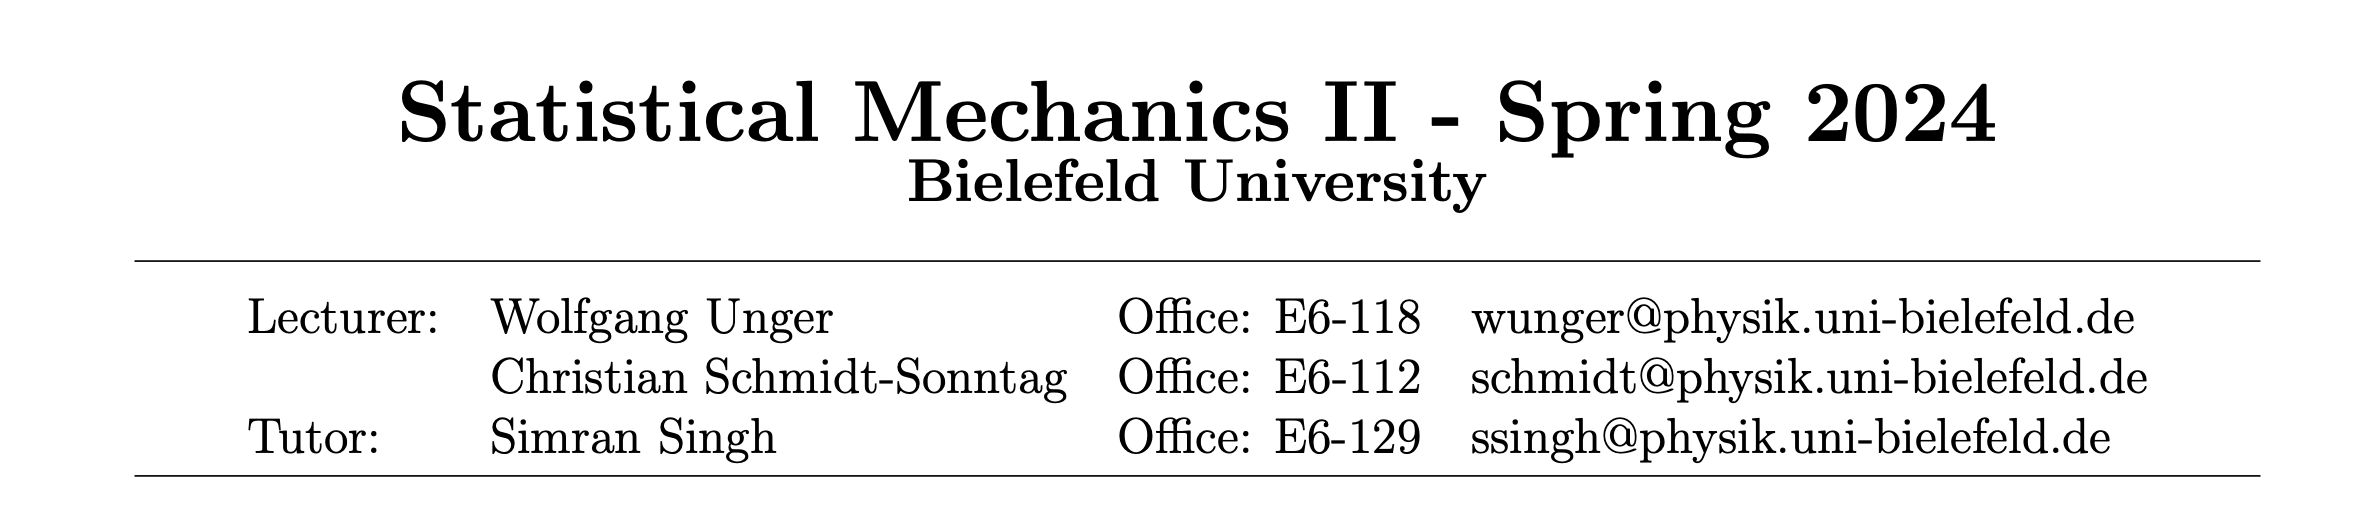
\includegraphics[scale=0.24]{exercise04.png}
\end{figure}
\hspace{4cm}\textbf{\Large{Exercise Nr 6 - part I}} \\
\vspace{-1cm}
\hspace{3cm}Discussion on June 4th , 16:00-18:00 in E6-124 

\vspace{2cm}

\noindent \textbf{15) Equivalence of boundary conditions} \\

\noindent In the lecture we derived the recursion relations in the absence of external magnetic field for the $1$D Ising model in the case of free boundary conditions and showed the result to be $Z^{(F)}_N = 2^N \prod_{i=1}^{N-1} \cosh(\beta J_i)$. 
\begin{enumerate}[i]
    \item Choosing uniform interactions \emph{i.e.,} $J_i = J \forall i$, derive the expressions for free energy, energy, specific heat. Are these functions analytic functions of $T,h$?
    \item From the beginning of the calculation, assuming \textbf{periodic} boundary conditions, derive the expression for the partition function. For finite number of lattice sites, this gives a different partition function than the free boundary case. Are they equivalent in the thermodynamic ($N \to \inft$) limit?
\end{enumerate}

\noindent \textbf{16) No phase transition in finite volume} \\
Representing the partition function as a polynomial in the fugacity variable and using the location of the Lee-Yang zeros, argue why there cannot be a phase transition in finite volume. \\

\noindent \textbf{17) Density of zeros near $T_c$} \\ Show that the density of zeros $g(\theta)$ behaves as $\theta^{1/\delta}$ near the origin $\theta=0$ at the critical point $T=T_c$ \footnote{This is exercise 9.10 from the book by Nishimori and Ortiz, which is freely available online. Hints are provided along with the exercise in the book}. 
\end{document}